\section{Digital-Analog-Wandler (DAC)}

\begin{minipage}[c]{0.42\columnwidth}
    \begin{tabular}{ll}
        $n$ & Anzahl Bits               \\
        $D$ & Digitaler Wert $D < 2^n$  \\
        $q$ & Quantisierungsschritt
  \end{tabular}
\end{minipage}
\hfill
\begin{minipage}[c]{0.54\columnwidth}
    $$ \boxed{ q = \frac{V_{\rm refp} - V_{\rm refn}}{2^n} } $$
    $$ \boxed{ V_{\rm out} =  \frac{D}{2^n} \, (V_{\rm refp} - V_{\rm refn}) + V_{\rm refn} } $$
\end{minipage}


\subsection{Parallelverfahren}

\subsubsection{Voltage Scaling - String DAC (3 Bit)}


\begin{minipage}[c]{0.15\columnwidth}
    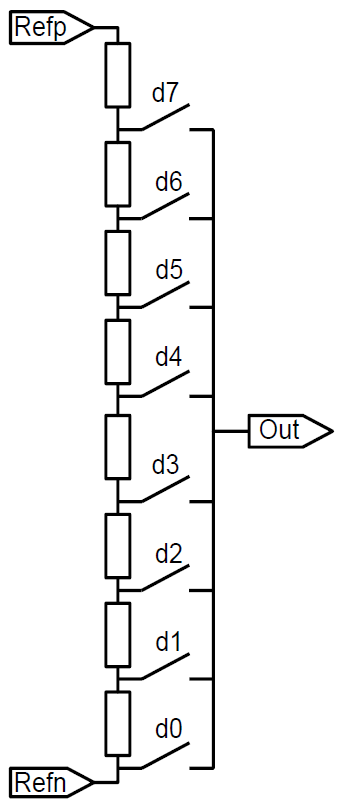
\includegraphics[height=3cm]{images/string_DAC.png}	% naja...
\end{minipage}
\hfill
\begin{minipage}[c]{0.8\columnwidth}
    Jeweils nur \textbf{ein Schalter} geschlossen

    \vspace{0.1cm}

    \begin{minipage}[c]{0.48\columnwidth}
        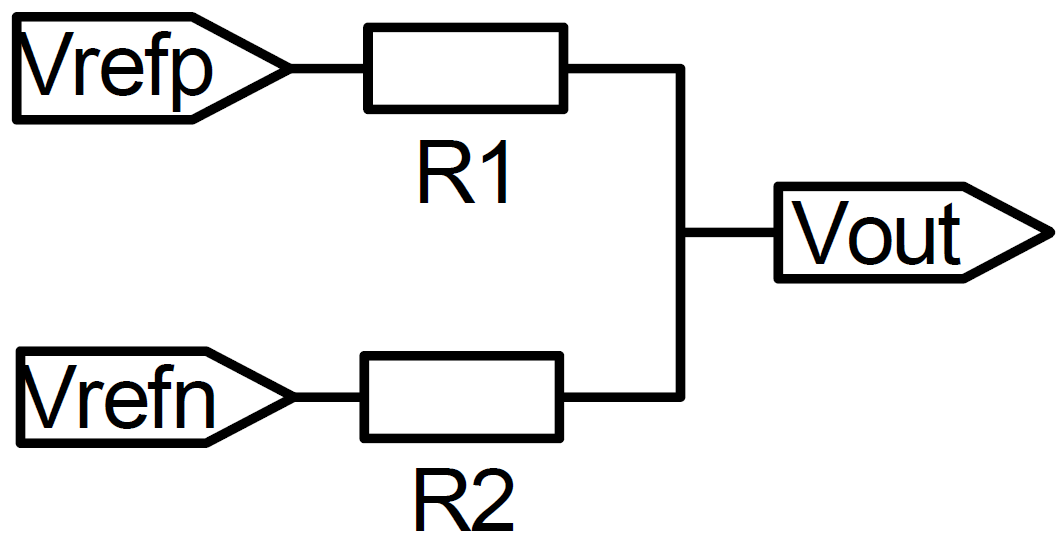
\includegraphics[width=0.95\columnwidth]{images/string_DAC_ersatzschaltung.png}
    \end{minipage}
    \hfill
    \begin{minipage}[c]{0.48\columnwidth}
        $R_1$: 1R \ldots 8R                                 \\
        $R_2$: 0R \ldots 7R                                 \\
        $V_{\rm out_{min}} = V_{\rm refn}$                  \\
        $V_{\rm out_{max}} = V_{\rm refp} - 1 \text{ LSB}$ 
    \end{minipage}

    \vspace{0.1cm}

    \begin{itemize}
        \item[+] Garantiert Stetigkeit
        \item $2^n$ Widerstände, $2^n$ Schalter \textrightarrow\ $n-\mathrm{to}-2^n$ Decoder
    \end{itemize}
\end{minipage}


\subsubsection{Voltage Scaling - String DAC (3 Bit)}

\begin{minipage}[c]{0.22\columnwidth}
    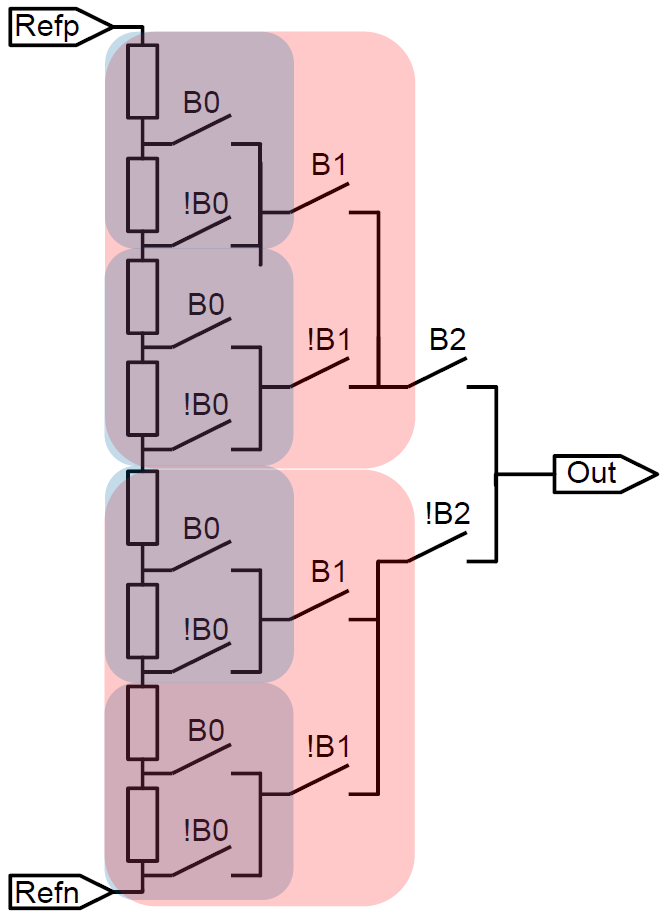
\includegraphics[width=\columnwidth]{images/string_DAC_advanced.png}
\end{minipage}
\hfill
\begin{minipage}[c]{0.76\columnwidth}
    Benötigt keinen Decoder aber zusätzliche Schalter

    \vspace{0.2cm}

    3-Bit DAC besteht aus: 

    \vspace{0.1cm}

    \begin{itemize}
        \item \cvt{4 mal 1-Bit DAC in Serie} 
        \item \crd{2 mal 2-Bit DAC in Serie}
    \end{itemize}

    \vspace{0.1cm}

    \textrightarrow\ Mit 2 mal 3-Bit DAC und Umschalter wird 4-Bit DAC gebaut
\end{minipage}


\subsubsection{Strom-DAC nach Parallelverfahren}

\begin{minipage}[c]{0.48\columnwidth}
    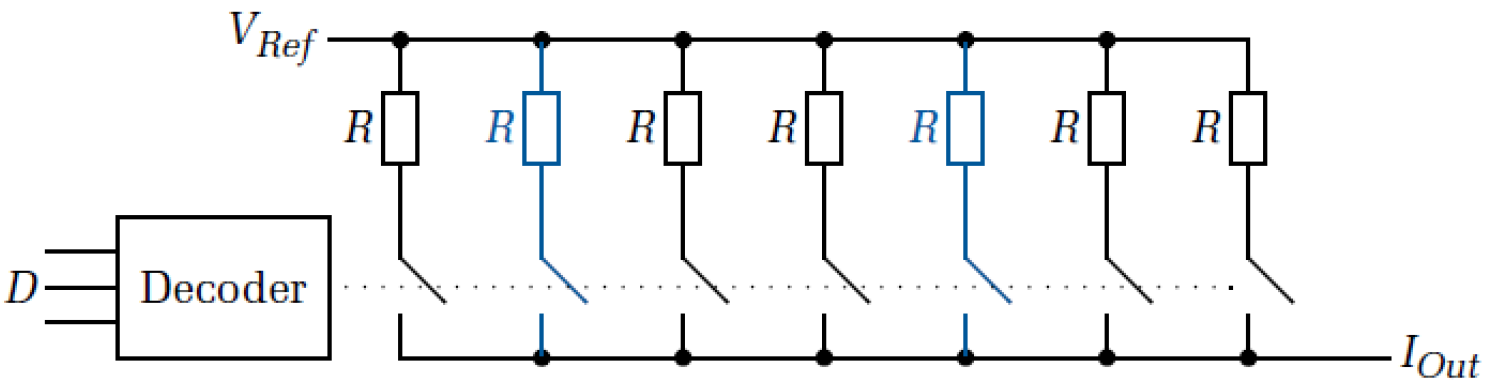
\includegraphics[width=\columnwidth]{images/strom_DAC_widerstaende.png} 
    $$ \boxed{ I_{\rm out} = D \frac{V_{\rm ref}}{R} } $$
\end{minipage}
\hfill
\begin{minipage}[c]{0.48\columnwidth}
    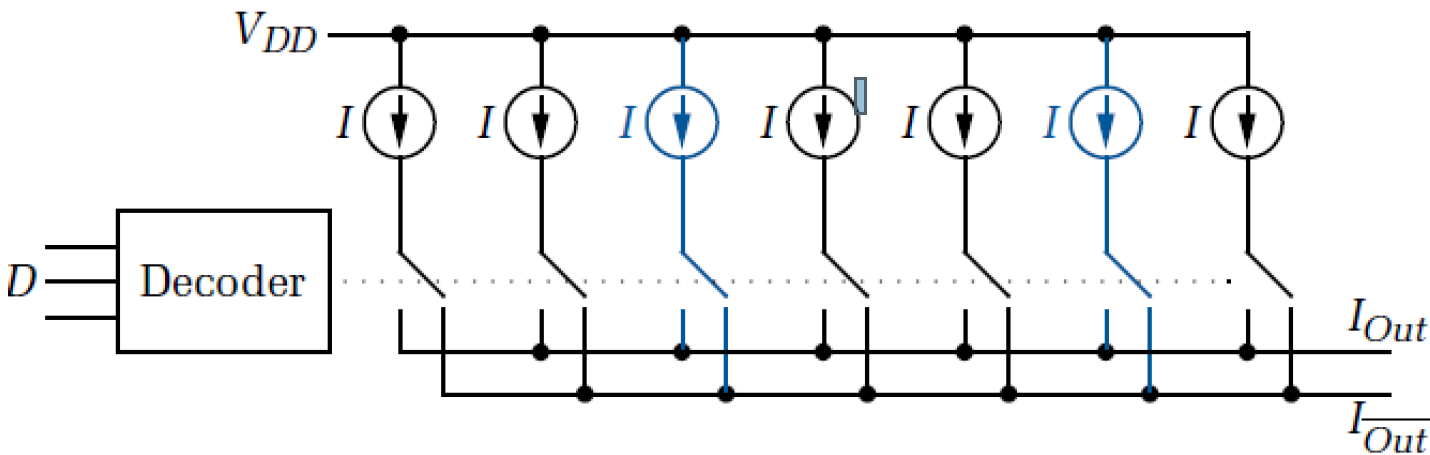
\includegraphics[width=\columnwidth]{images/strom_DAC_stromquellen.png}
    $$ \boxed{ I_{\rm out} = D \cdot I } $$
\end{minipage}

\vspace{0.2cm}

Um eine Ausgangsspannung $V_{\rm out}$ zu erhalten, wird ein OPV nachgeschaltet gemäss Kapitel \ref{R2R}

\columnbreak


\subsection{Wägeverfahren}

\subsubsection{Wägeverfahren -- resistiv}

\begin{minipage}[c]{0.4\columnwidth}
    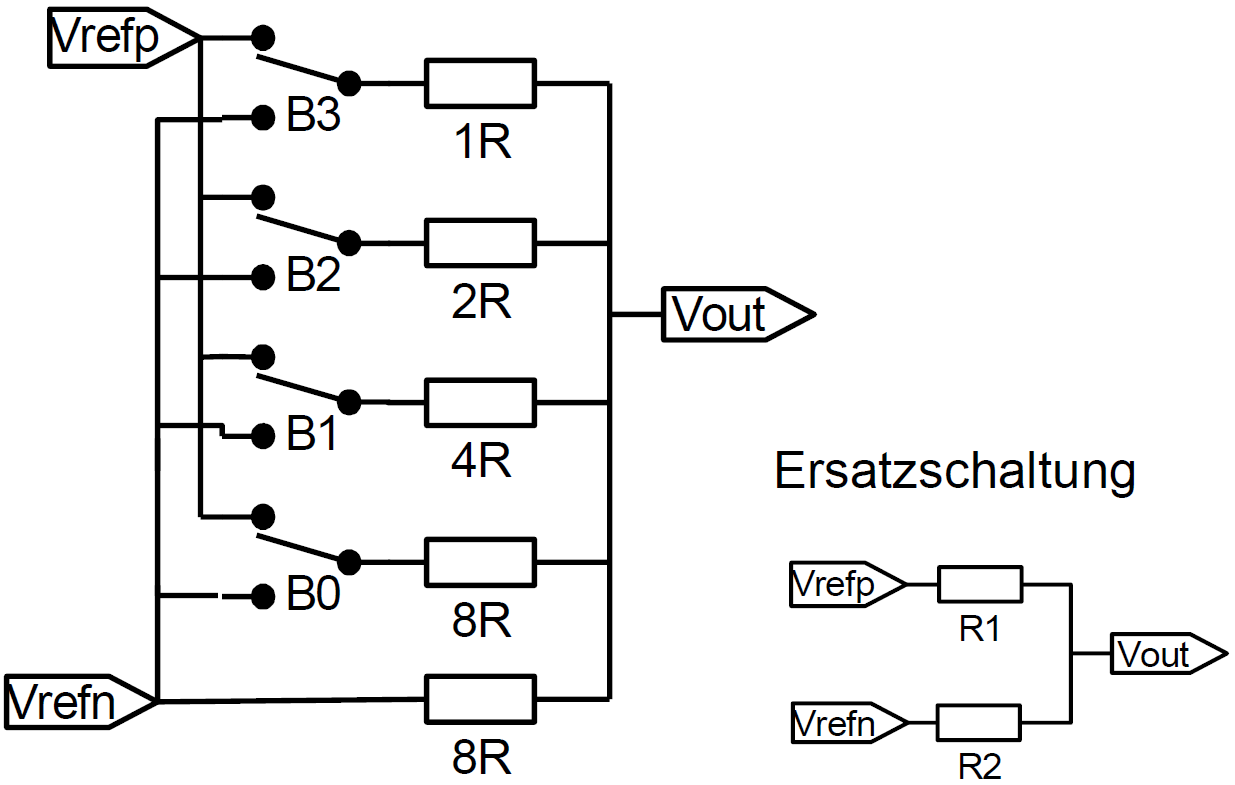
\includegraphics[width=\columnwidth]{images/waegeverfahren.png}
\end{minipage}
\hfill
\begin{minipage}[c]{0.53\columnwidth}
    \begin{itemize}
        \item[+] $N$ Widerstände, $N$ Schalter 
        \item[-] Nicht garantiert stetig
        \item[-] Grosser Wertebereich der Widerstände nötig 
    \end{itemize}

    $$ \textbf{Leitwerte!} \qquad \bm{G_0 = \frac{1}{8R} } $$
\end{minipage}

$$ \boxed{ V_{\rm out} = \frac{B_0 \cdot 2^0 \cdot G_0 + B_1 \cdot 2^1 \cdot G_0 + B_2 \cdot 2^2 \cdot G_0+ B_3 \cdot 2^3 \cdot G_0}{2^4 \cdot G_0} (V_{\rm refp}- V_{\rm refn}) + V_{\rm refn} } $$


\subsubsection{Kapazitiver DAC ohne Ausgangsbuffer (4 Bit)}

\begin{center}
    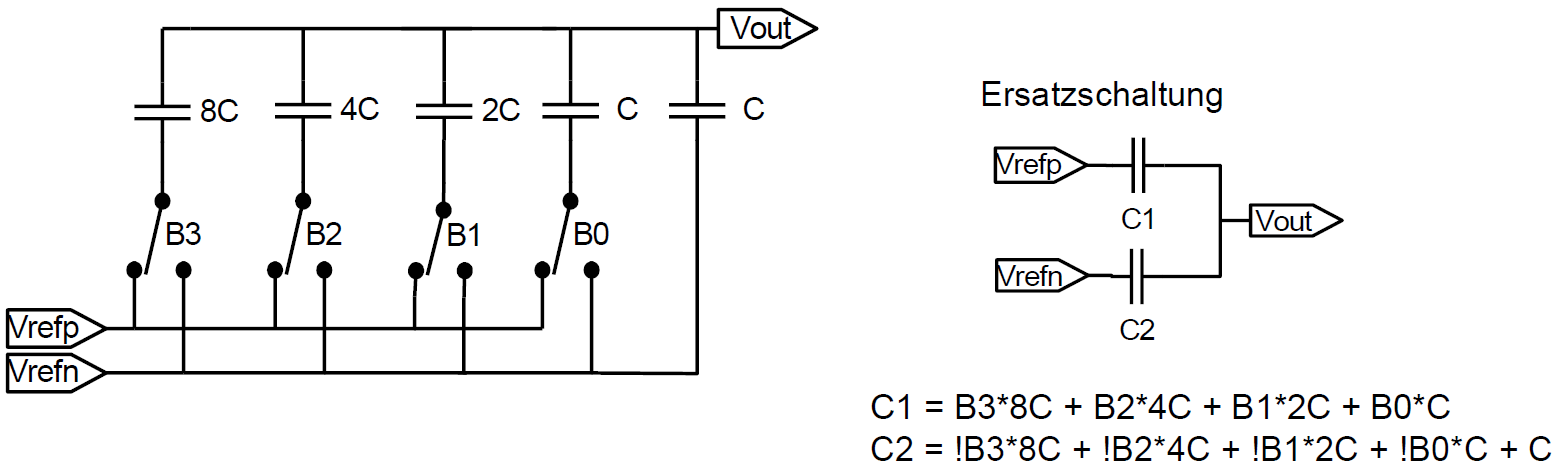
\includegraphics[width=0.85\columnwidth]{images/kapazitiver_DAC_2.png}
\end{center}

Wenn Kapazitäten entladen sind, bevor geschaltet wird: 
$$ \boxed{ V_{\rm out} = \frac{C_1}{C_1 + C_2} (V_{\rm refp} - V_{\rm refn}) + V_{\rm refn}  \quad  \text{mit } C_1 + C_2 = 2^n \cdot C } $$

\textbf{Problem:} Lastkapazitäten an $V_{\rm out}$ \textrightarrow\ Schaltung so schlecht brauchbar  


\subsubsection{Kapazitiver DAC mit Ausgangsbuffer}

\begin{minipage}[c]{0.4\columnwidth}
    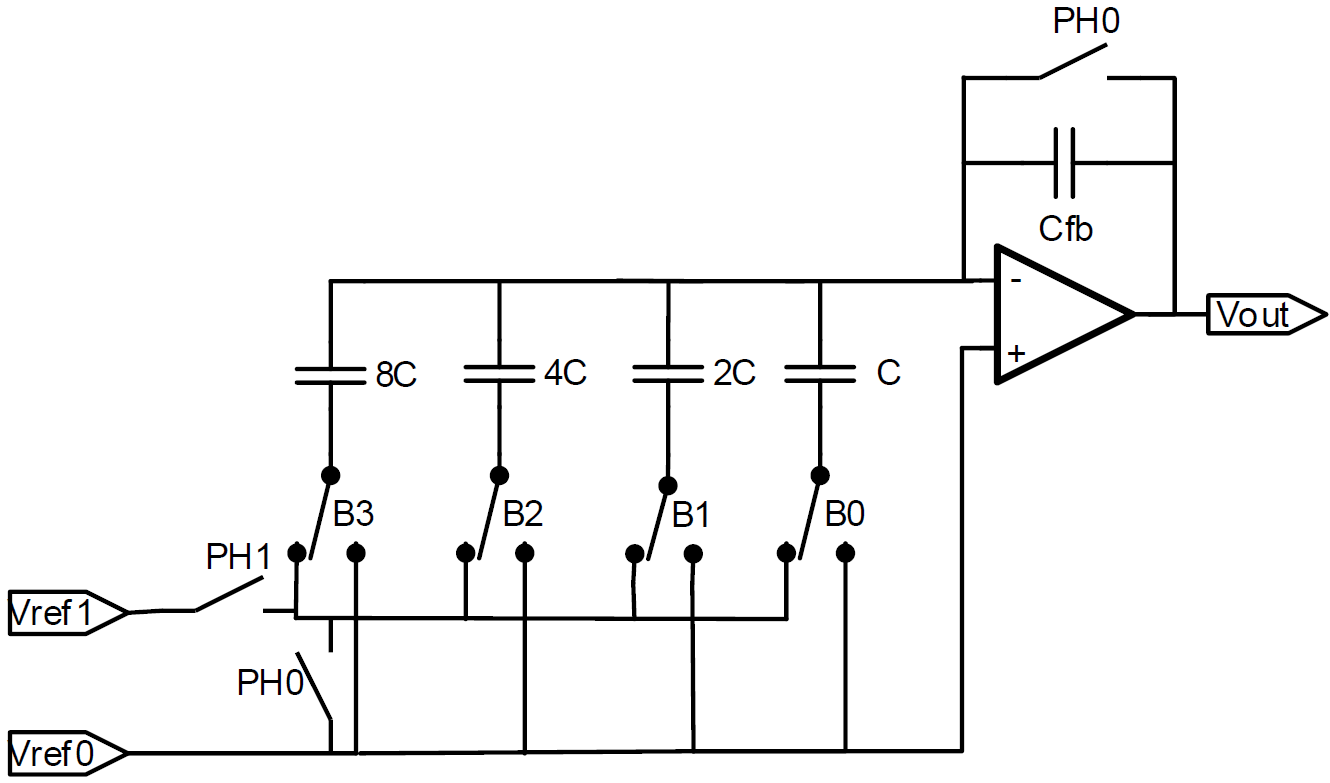
\includegraphics[width=\columnwidth]{images/kapazitiver_DAC_ausgangsbuffer.png}
\end{minipage}
\hfill
\begin{minipage}[c]{0.53\columnwidth}
    \raggedright
    Immer nur ein Schalter geschlossen! \\
    2 Phasen: PH0 und PH1 

    \vspace{0.2cm}
    PH0: $V_{\rm out} = V_{\rm ref0}$ \\
    PH1: Ausgang gültig (nach Einschwingen)

    $$ \boxed{ V_{\rm out} = -(V_{\rm ref1} - V_{\rm ref0}) \cdot \Bigg( \frac{n \cdot C}{C_{fb}}  \Bigg) + V_{\rm ref0} } $$
\end{minipage}

\vspace{0.2cm}

\textbf{Nachteil:} Sample-Hold nötig für Ausgangsspannung in Phase PH0 (wenn Schalterstellung gewechselt wird)


\subsubsection{Wägeverfahren mit Widerständen und Ausgangsverstärker}

\begin{minipage}[c]{0.45\columnwidth}
    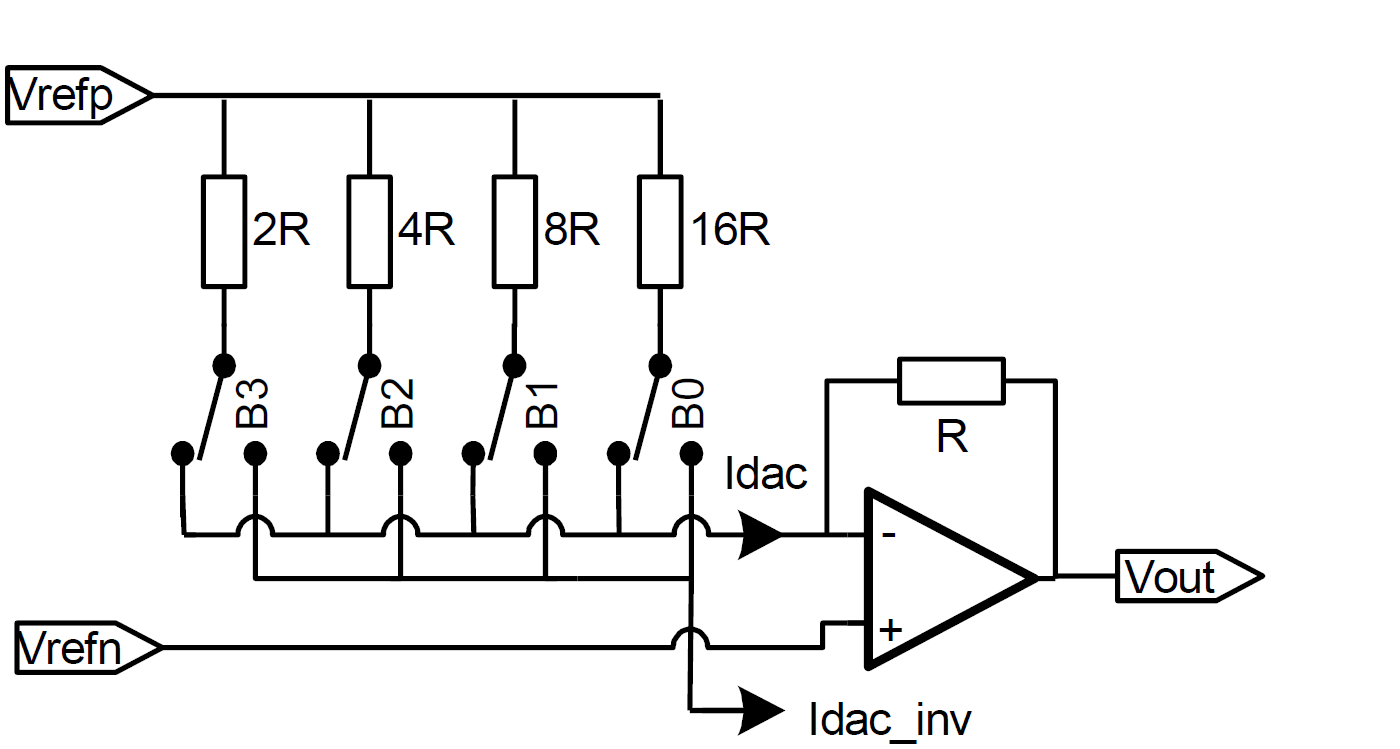
\includegraphics[width=\columnwidth]{images/DAC_ausgangsverstaerker.png}
\end{minipage}
\hfill
\begin{minipage}[c]{0.53\columnwidth}
    $$ \boxed{ I_{\rm dac_{max}} = \frac{V_{\rm refp} - V_{\rm refn}}{R} \frac{2^n -1}{2^n} } $$
    $$ \boxed{ I_{\rm dac} = \frac{V_{\rm refp} - V_{\rm refn}}{R} \frac{D}{2^n}  } $$
    $$ \boxed{ V_{\rm out} = V_{\rm refn} - R \cdot I_{\rm dac} } $$

    \vspace{0.2cm}
    \begin{itemize}
        \item[+] differentiell ($I_{\rm dac_{inv}}$)
        \item[-] Ausgang darf belastet werden
    \end{itemize}
\end{minipage}


\subsubsection{DAC mit R2R-Netzwerk}
\label{R2R}

\begin{minipage}[c]{0.4\columnwidth}
    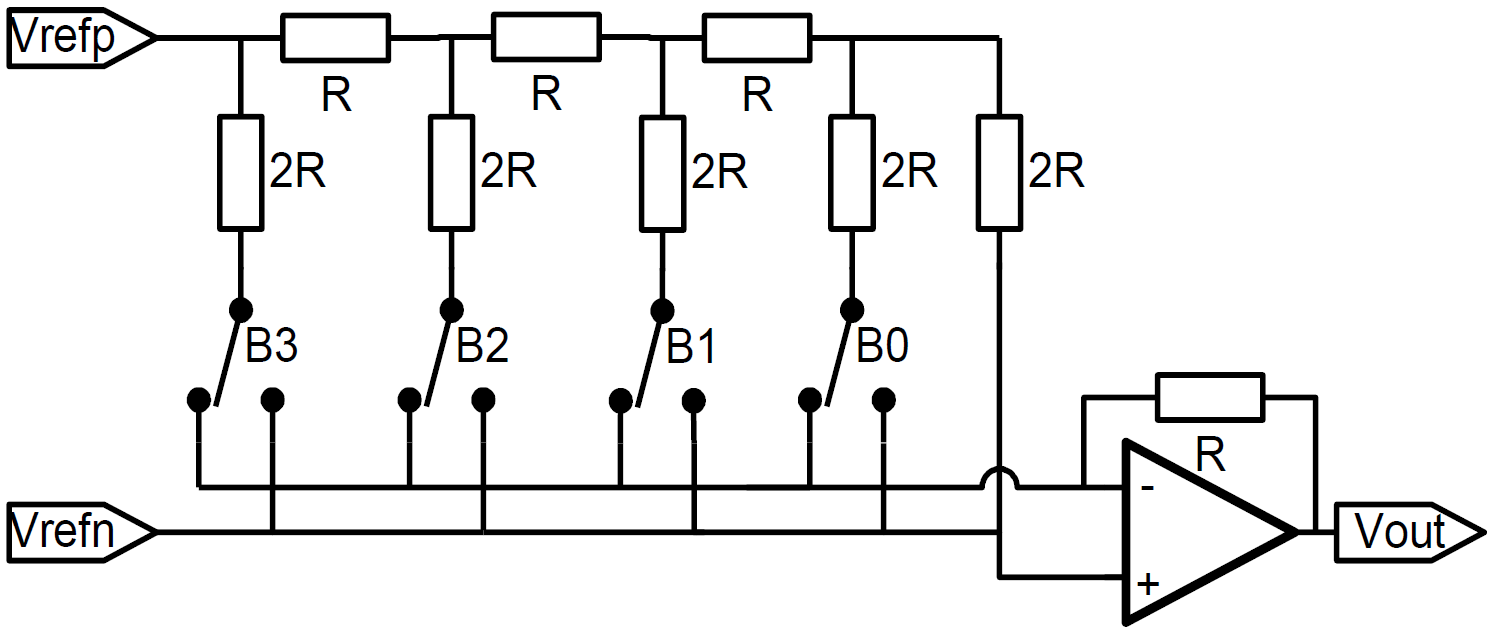
\includegraphics[width=\columnwidth]{images/R2R_netzwerk}
\end{minipage}
\hfill
\begin{minipage}[c]{0.56\columnwidth}
    Für Ersatzwiderstand \textbf{von rechts} her 'schauen'

    \vspace{0.2cm}
    
    \begin{itemize}
        \item[+] Nur 2 Widerstandswerte: R, 2R
        \item[+] Gute Alternative zu gewichteten R's bzw. C's
        \item[+] Stromgewichtung über Spannungsteiler von $V_{\rm refp}$ zu $V_{\rm refn}$
    \end{itemize}
\end{minipage}

\vspace{0.2cm}
Variiert $V_{\rm refp}$, dann variiert auch $V_{\rm out}$

\textbf{Jeder geschlossene Schalter trägt gewichtet zur Ausgangsspannung bei! \\
Achtung: Invertierung!}

$$ \boxed{V_{\rm out} = V_{\rm refn} - (V_{\rm refp} - V_{\rm refn}) \cdot \frac{D}{2^n}}  $$


\cbl{\myul{\textbf{Beispiel:}}

\renewcommand{\arraystretch}{1.8}
\begin{tabular}{lll}
    $B_3 \text{ geschlossen: } V_{\rm out} = V_{\rm refn} - \frac{\Delta V_{\rm ref}}{2}$    & & 
    $B_2 \text{ geschlossen: } V_{\rm out} = V_{\rm refn} - \frac{\Delta V_{\rm ref}}{4}$    \\
    $B_1 \text{ geschlossen: } V_{\rm out} = V_{\rm refn} - \frac{\Delta V_{\rm ref}}{8}$    & & 
    $B_0 \text{ geschlossen: } V_{\rm out} = V_{\rm refn} - \frac{\Delta V_{\rm ref}}{16}$
\end{tabular}
}
\renewcommand{\arraystretch}{1}


\subsection{Einschub: Kapazitiver Spannungsteiler}

\begin{minipage}[c]{0.4\columnwidth}
    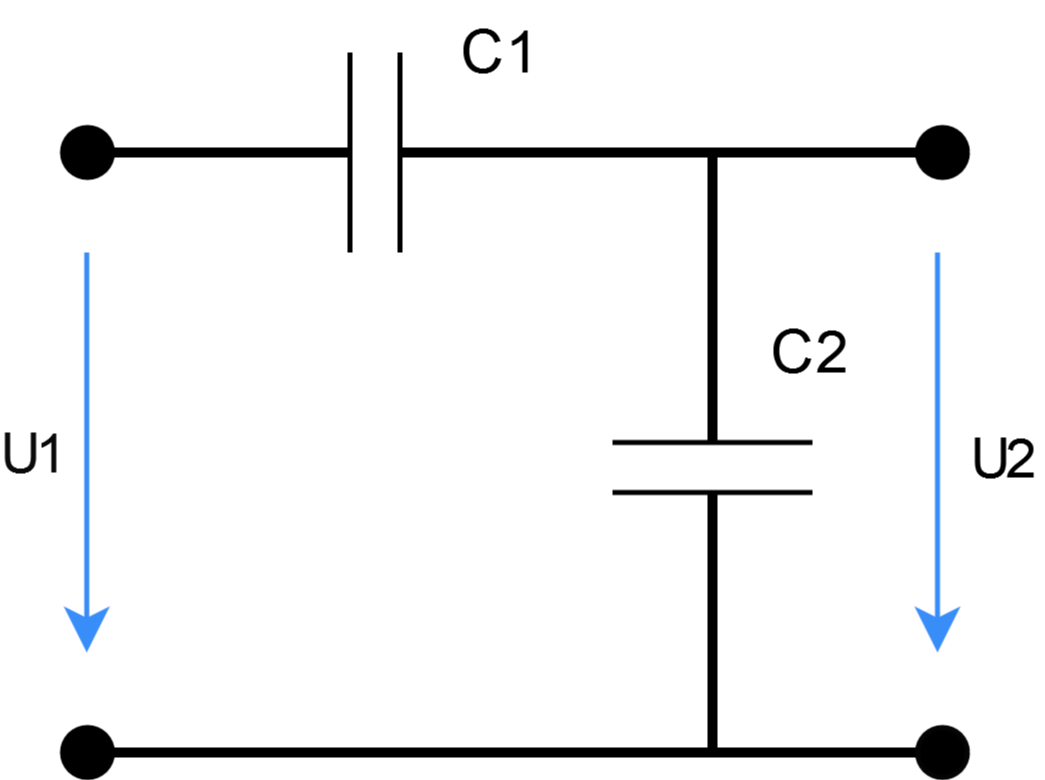
\includegraphics[width=0.7\columnwidth]{images/CapSpannungsteiler.png} 
\end{minipage}
\hfill
\begin{minipage}[c]{0.58\columnwidth}
    $$ \boxed{ U_2 = U_1 \cdot \frac{X_2}{X_1 + X_2} = U_1 \cdot \frac{C_1}{C_1 + C_2} } $$
\end{minipage}


\subsection{Zählverfahren (PWM)}

\subsubsection{PWM: Pulse Width Modulation}

\begin{minipage}[c]{0.45\columnwidth}
    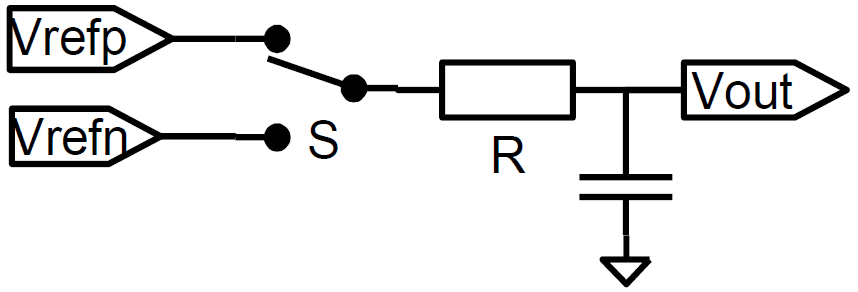
\includegraphics[width=\columnwidth]{images/PWM_DAC}
\end{minipage}
\hfill
\begin{minipage}[c]{0.52\columnwidth}
    \raggedright
    $S$ schaltet zwischen $V_{\rm refp}$ und $V_{\rm refn}$ (\textrightarrow\ PWM) \\
    (\textrightarrow\ meistens $V_{\rm ref}$ und $GND$ )

    \vspace{0.2cm}

    \textbf{RC glättet und erzeugt 'DC'}
\end{minipage}

\vspace{0.2cm}

\begin{minipage}[c]{0.48\columnwidth}
    \begin{itemize}
        \item[+] Sehr einfache Schaltung
        \item[+] Ermöglicht hohe Auflösung 
        \item[+] Funktioniert onchip digital (z.B. FPGA, $\mu$C) \textrightarrow\ analoge Schaltung extern
    \end{itemize}
\end{minipage}
\hfill
\begin{minipage}[c]{0.48\columnwidth}
    \raggedright
    \begin{itemize}
        \item[-] Sehr langsam
        \item[-] Benötigt grosses $\tau$ für kleine Spannungsrippel (oder Tiefpass höherer Ordnung)
    \end{itemize}
\end{minipage}

\vspace{0.2cm}

\myul{\textbf{PWM-Ansteuerung für Schalter $\bm{S}$}}

\vspace{0.1cm}

\begin{minipage}[c]{0.4\columnwidth}
    $$ \boxed{ \overline{V_{\rm out}} = V_{\rm ref} \cdot \frac{n}{N} }  $$
\end{minipage}
\hfill
\begin{minipage}[c]{0.58\columnwidth}
    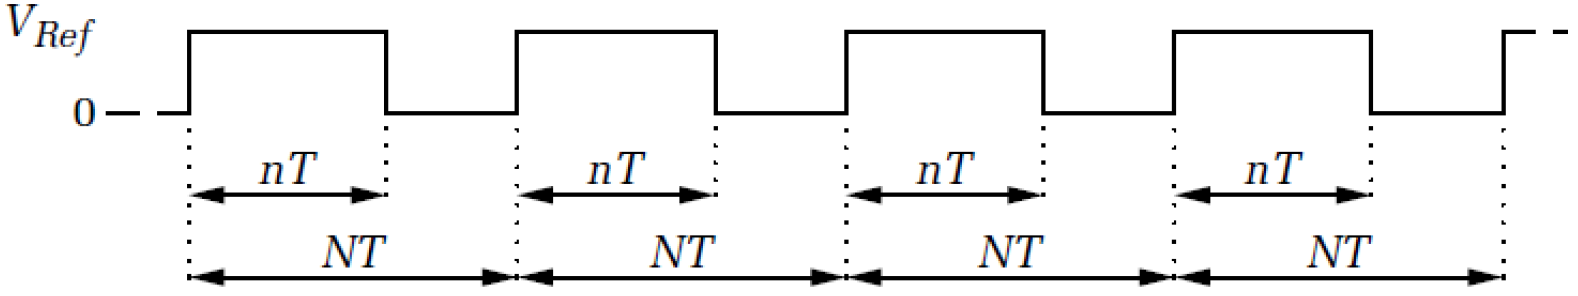
\includegraphics[width=\columnwidth]{images/PWM_ansteuerung_2.png} 
\end{minipage}


\subsection{Kaskadierte Wandler und Mischformen}

\subsubsection{Kaskadierte DACs}

\begin{minipage}[c]{0.6\columnwidth}
    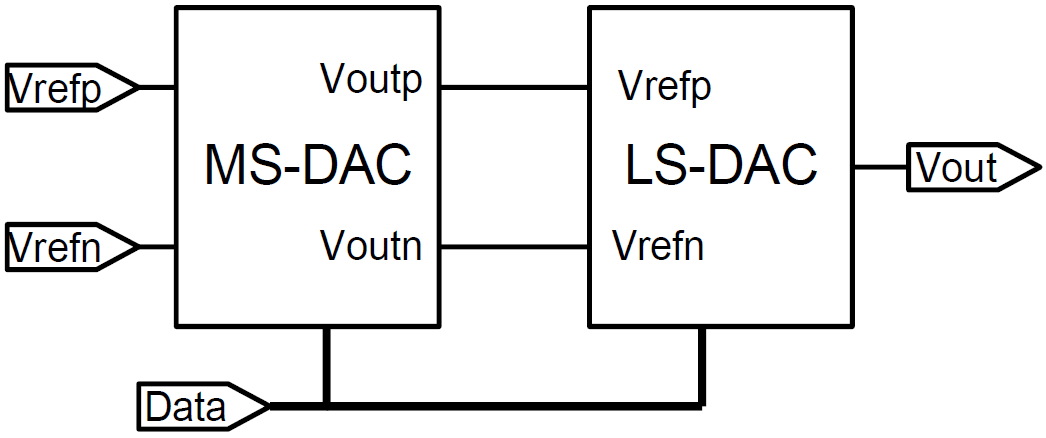
\includegraphics[width=0.75\columnwidth]{images/kaskadierte_DAC_1.png}
\end{minipage}
\hfill
\begin{minipage}[c]{0.38\columnwidth}
    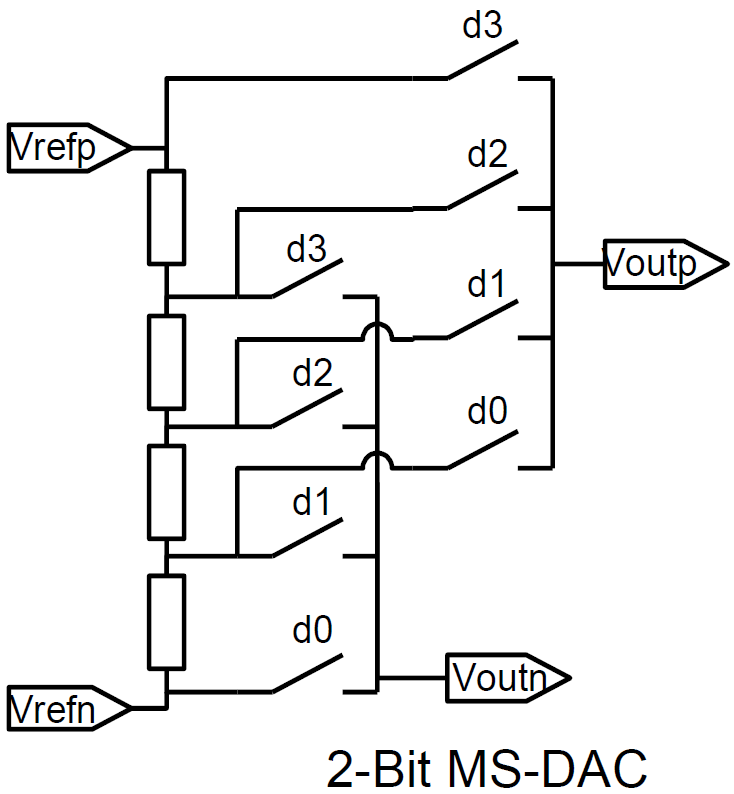
\includegraphics[width=0.7\columnwidth]{images/kaskadierte_DAC_2.png}
\end{minipage}

\vspace{0.2cm}

\begin{itemize}
    \item MS-DAC: 2 Ausgangsspannungen (über / unter gewünschtem $V_{\rm out}$)
    \item LS-DAC: folglich kleinere Eingangsspannungsdifferenz \\
        \textrightarrow\ Kleinerer Quantisierungsschritt $q$ \\
        \textrightarrow\ Höhere absolute Spannungsauflösung
\end{itemize}


\subsubsection{Segmentierter String DAC}

\begin{minipage}[c]{0.3\columnwidth}
    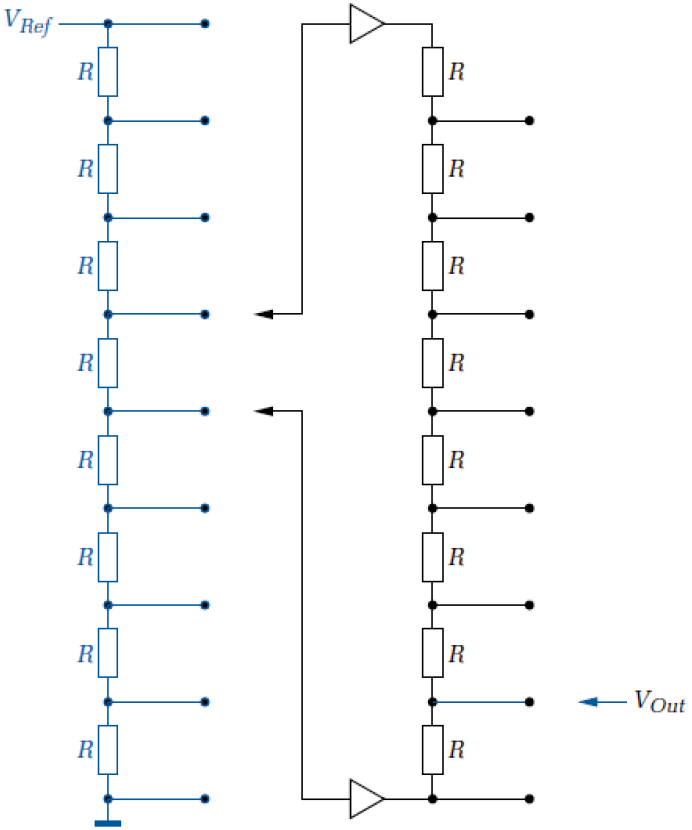
\includegraphics[width=\columnwidth]{images/segmented_string.png} 
\end{minipage}
\hfill
\begin{minipage}[c]{0.68\columnwidth}
    \begin{itemize}
        \item 2 'Strings' mit tiefer Auflösung ergeben doppelte\\
            Auflösung \textrightarrow\ $2 \cdot 8$R \textrightarrow\ $2 \cdot 3$ Bit
        
        \vspace{0.2cm}

        \item[+] Viel weniger Elemente
        \item[-] Benötigt 2 Buffer (damit keine Belastung des linkes 'Strings')
        \item[-] Buffer müsste offset-frei sein
    \end{itemize}

    \vspace{0.2cm}

    Alternative: Viel grössere R in rechtem 'String' \\
    \textrightarrow\ kleine Belastung links
\end{minipage}


\subsection{Zusammenfassung DACs}

    \begin{tabular}{ll}
    Parllelverfahren    & ... garantiert monotone Wandler           \\
    Wägeverfahren       & ... Anzahl Elemente nicht allzu hoch      \\
    Zählverfahren       & ... Wenn Zeit untergrodnete Rolle spielt
\end{tabular}

\vspace{0.2cm}

\textrightarrow\ \textbf{Oft werden Parallel- und Wägeverfahren kombiniert!}

\vspace{0.1cm}

Schnelle DACs haben oft einen Stromausgang und benötigen daher einen Ausgangsverstärker
\textrightarrow\ Ströme können schneller geschaltet werden als Spannungen!

\vspace{0.2cm}

Es gilt: Für optimale Resultate müssen \textbf{Kompromisse} eingegangen werden! 
